\documentclass[11pt,a4paper]{article}

\usepackage[utf8]{inputenc}
\usepackage[T1]{fontenc}
\usepackage{lmodern}
\usepackage[margin=2.5cm]{geometry}
\usepackage{fancyhdr}
\usepackage{titlesec}
\usepackage{xcolor}
\usepackage{booktabs}
\usepackage{graphicx}
\usepackage{amsmath}
\usepackage{float}
\usepackage{caption}
\usepackage{enumitem}
\usepackage[colorlinks=true,linkcolor=navy,urlcolor=navy,citecolor=navy]{hyperref}

\definecolor{navy}{HTML}{1F3A5F}
\titleformat{\section}{\Large\bfseries\color{navy}}{\thesection.}{0.6em}{}
\titleformat{\subsection}{\large\bfseries\color{navy}}{\thesubsection.}{0.6em}{}
\captionsetup{font=small,labelfont=bf}
\setlist{itemsep=2pt}

\pagestyle{fancy}
\fancyhf{}
\lhead{BIG DATA}
\rhead{Assignment 4}
\cfoot{\thepage}
\renewcommand{\headrulewidth}{0.4pt}

\begin{document}

% ------------------------------------------------------------------ title page
\begin{titlepage}
\thispagestyle{empty}
\vspace*{1cm}
{\color{navy}\Large\bfseries BIG DATA}\\[2pt]
{\large Data Science and Engineering}\\[2pt]
{\large Academic Year 2026--2027}\\[2.5cm]

{\color{navy}\fontsize{30}{36}\selectfont\bfseries Distributed Matrix\\ Multiplication}\\[0.6cm]
{\Large Strong scaling of a Hazelcast implementation with local workers on an Apple M1}\\[2cm]

\textbf{Research focus}\\[4pt]
How does a Hazelcast-based dense matrix multiplication scale with the number of workers
when all workers run as separate JVM processes on one machine, and how large are the
framework and data-movement costs compared with a sequential and a multithreaded Java
baseline?\\[1.5cm]

\textbf{Student}\\ Zayra Penya Juan\\[0.8cm]
\textbf{Assignment}\\ Assignment 4 -- Distributed Matrix Multiplication\\[0.8cm]
\textbf{Submission}\\ November 2026
\end{titlepage}

\tableofcontents
\newpage
\listoffigures
\listoftables
\newpage

% ------------------------------------------------------------------ abstract
\section*{Abstract}
This report studies the strong scaling of a distributed dense matrix multiplication built
with Hazelcast, and compares it with a sequential and a multithreaded Java baseline that use
the same kernel and the same input matrices. A worker is a Hazelcast member, that is, a
separate JVM process with one compute thread. All workers run on a single MacBook Air (Apple
M1, 8 GB), so the experiment measures framework, serialization and process overhead, not
inter-machine network performance or multi-machine memory capacity.

Rows of $A$ are divided into one block per worker and shipped inside the tasks. $B$ is
uploaded to a distributed map and read by every task, and the blocks of $C$ are returned to
the driver. Sizes $n\in\{500,1000,1500,2000\}$ were run with $W\in\{1,2,4,8\}$ workers, five
measured repetitions per configuration after three warm-up runs, and medians and
interquartile ranges (IQR) are reported.

With one worker the distributed code is 4.3\% to 30.3\% slower than the sequential kernel
(30.3\% at $n=500$, 4.3\% at $n=2000$). The best speedup over one worker was $2.26\times$
($n=2000$, $W=4$); with eight workers the time was worse than with four for every size. The
best end-to-end speedup over the Java sequential kernel was $2.16\times$, and the distributed
version was never faster than Java threads on the same machine. Memory sampled across all
processes was between 9.5 and 21.9 times that of the sequential run for $n=2000$. Conclusions
are limited to this implementation, to local execution, and to this hardware.

\textbf{Keywords:} distributed computing, Hazelcast, matrix multiplication, strong scaling,
speedup, serialization overhead, Apple M1.

% ------------------------------------------------------------------ 1
\section{Introduction and objectives}
Distributed frameworks allow work and data to be spread across processes or machines, but the
benefit depends on how much computation each worker receives compared with the cost of moving
data and coordinating tasks. Dense matrix multiplication is a useful test case: the
arithmetic is $O(n^3)$ while the data is $O(n^2)$, so the ratio of computation to data
movement improves with $n$.

The research questions are:
\begin{itemize}
  \item How does the end-to-end time of the distributed implementation change with the
        number of workers for a fixed problem size (strong scaling)?
  \item How large is the overhead of the framework with one worker compared with the
        sequential Java kernel?
  \item How do the distributed version and the multithreaded Java version compare on the
        same machine?
  \item Which parts of the execution (data upload, computation, result collection) account
        for the observed times, and what do the memory measurements show?
\end{itemize}
Hypothesis: with workers on one machine, the distributed version should scale until the
number of processes exceeds the available execution contexts and should not beat threads in a
single process, because every worker pays for serialization and inter-process communication
that threads avoid. Weak scaling was not studied.

% ------------------------------------------------------------------ 2
\section{Background and references}
For square matrices $A$ and $B$ of dimension $n$, $C=AB$ with
$C_{ij}=\sum_{k=0}^{n-1}A_{ik}B_{kj}$. The i--k--j kernel from the earlier assignments is
used on every worker.

Hazelcast provides distributed data structures and a distributed executor service. The
distributed map \texttt{IMap} is a concurrent, distributed map \cite{hz-imap}; the reference
manual describes how its data is distributed over the members, with optional backup copies
controlled by the backup count \cite{hz-map-guide}. The executor service \texttt{IExecutorService} runs \texttt{Callable}
tasks on a chosen member and returns a \texttt{Future} \cite{hz-exec}. This study uses these
two pieces.

Speedup and efficiency are defined as in the previous assignment. For a fixed problem size
and $W$ workers,
\[
  S(W)=\frac{T_{\mathrm{ref}}}{T_W},\qquad E(W)=\frac{S(W)}{W},
\]
where $T_{\mathrm{ref}}$ is either the time with one distributed worker (strong scaling inside
the framework) or the sequential Java kernel time (comparison with the baseline); both are
medians and each table states which reference is used. Amdahl's argument is that a fixed
problem has a limit to its speedup when part of the work does not parallelise \cite{amdahl}.
Gustafson noted that this assumes a fixed problem size and described a scaled-size view
\cite{gustafson}; only the fixed-size (strong scaling) view is studied here.

% ------------------------------------------------------------------ 3
\section{Methodology}
\subsection{Environment and settings}
\begin{table}[H]
\centering
\caption{Experimental environment (all measurements on one machine).}
\begin{tabular}{@{}ll@{}}
\toprule
Parameter & Configuration \\
\midrule
Machine & MacBook Air, Apple M1, one physical machine \\
CPU cores & 8 physical, 8 logical: 4 performance + 4 efficiency \\
Memory & 8 GB RAM \\
Operating system & macOS 14.6.1 (Darwin 23.6.0, arm64) \\
Java & OpenJDK 25.0.2 (bytecode compiled with \texttt{release 11}) \\
Framework & Hazelcast 5.3.8 (Community, from Maven) \\
Build & Apache Maven 3.9.16, shaded jar \\
Workers & Hazelcast members: one JVM process each, executor with 1 thread \\
Worker counts & 1, 2, 4, 8 (plus one client JVM for the driver) \\
JVM heap & members \texttt{-Xmx1g}, driver and baselines \texttt{-Xmx3g} \\
Network & loopback (127.0.0.1), TCP-IP join, multicast disabled \\
Date of the run & 22 November 2026 \\
Power source & battery (reported by \texttt{pmset} at run time) \\
Repetitions & 5 measured, 3 warm-up (excluded; JIT) \\
Per-configuration budget & 300 s (none exceeded) \\
\bottomrule
\end{tabular}
\end{table}
The label of this environment is \emph{local execution}: the ``workers'' are processes on one
machine, they share the same CPU, caches, memory and operating system, and the network is the
loopback interface. Hazelcast 5.3.8 prints warnings about \texttt{sun.misc.Unsafe} with this
Java version; they appear in the output, and their effect on performance was not evaluated.

\subsection{Implementations}
\begin{itemize}
  \item \textbf{Sequential (seq):} i--k--j kernel in one thread of one JVM.
  \item \textbf{Java threads (par):} same kernel, rows of $C$ split into $p$ blocks, one Java
        thread per block, in a single JVM. Thread creation and joining are inside the timer.
  \item \textbf{Distributed (dist):} $W$ Hazelcast members, one row block of $A$ per member.
\end{itemize}
The distributed algorithm has three steps. (1)~The driver, a Hazelcast client, slices $B$
into 16 row panels and uploads them with \texttt{putAll} to an \texttt{IMap} (no backup
copies, so each panel is stored once). (2)~For each worker, the driver sends one task to that
member (\texttt{submitToMember}); the row block of $A$ travels inside the task. The task reads
all 16 panels of $B$ from the map, assembles $B$ locally, runs the kernel and returns its block
of $C$ as the result. (3)~The driver copies the returned blocks into the full $C$. Computation
therefore takes place on the members, $B$ is stored distributed, $A$ and $C$ move between
driver and members, and the result is collected at the driver. The code is in the repository
(Section~\ref{sec:repro}).

\subsection{Inputs}
Matrices are generated with the splitmix64 generator \cite{splitmix}, values in $[0,1)$, with
seeds $\mathrm{seed}_A=42+17n$ and $\mathrm{seed}_B=\mathrm{seed}_A+1000003$. The same
generator and seeds were used in Assignment~3 (C). The checksums of the Java sequential result
and of the C sequential result of Assignment~3 are equal for all four sizes (relative
difference 0), so the logical inputs are the same.

\subsection{Timing protocol}
Inputs are generated and the output arrays are allocated outside the timed region.
\begin{itemize}
  \item \textbf{seq and par:} the timer covers the kernel only. The kernel zeroes the
        output rows inside the timed region, and for par thread creation and joining are
        included.
  \item \textbf{dist:} the end-to-end time covers three consecutive phases at the driver:
        (a)~slicing and uploading $B$; (b)~the compute phase, from the first task submission
        until all results have been received, which includes slicing and sending the blocks of
        $A$, reading $B$ on the members, the kernel and the return of $C$; (c)~assembly of
        $C$ at the driver. Because they are consecutive, the three phases add up to the
        end-to-end time.
\end{itemize}
Inside each task the program also measures the time to read and assemble $B$
(\texttt{max\_fetch}) and the kernel time (\texttt{max\_kernel}), reported as the maximum over
the tasks of a run. These in-task times \emph{overlap} the compute phase and run in parallel on
different members, so they are not added to the phase times. The map is cleared after each
repetition, so every repetition uploads $B$ again. A monotonic clock (\texttt{nanoTime}) is
used, and the sum of $C$ is computed outside the timer so that the result is used.

Comparisons between the distributed version and the baselines use the end-to-end time of the
distributed version and the kernel time of the baselines; this is stated in each table and
should be read as a comparison between a complete distributed run and a kernel run, not between
identical boundaries.

\subsection{Correctness}
Tests ran with 1, 2 and 3 workers for $n\in\{1,2,3,7,16,33,100\}$ (including more blocks than
rows), with identity and zero matrices, and compared the distributed result with the
sequential kernel and the sequential kernel with a naive i--j--k reference. All tests passed:
the maximum absolute difference between distributed and sequential results was 0 (identical
bitwise), the maximum relative error between sequential and naive was 0, and the multithreaded
result equals the sequential one. The result of every repetition is reduced to a checksum
stored in the raw data.

\subsection{Memory and data transfer}
Memory is measured by sampling the resident set size (RSS) of each process with \texttt{ps}
every 0.2\,s. The report uses the maximum over samples of the sum over all processes of a
configuration (total), and the maxima of the driver and of any member. This is a sampled
value, not a true peak, and very short runs have few samples. The amount of transferred data
was not measured; Section~\ref{sec:results} uses an analytical estimate computed from the
sizes (the payload of $B$ upload, $A$ blocks, $B$ reads by each task and $C$ blocks is
$(3+W)\cdot 8n^2$ bytes), which is not a measurement and is not network traffic between
machines.

% ------------------------------------------------------------------ 4
\section{Results}\label{sec:results}
\subsection{Baselines}
\begin{table}[H]
\centering
\caption{Java baselines: median kernel time in seconds (5 repetitions). The sequential IQR is at most 0.00046\,s.}
\small
\begin{tabular}{@{}rrrrrr@{}}
\toprule
$n$ & seq & par $p=1$ & par $p=2$ & par $p=4$ & par $p=8$ \\
\midrule
500  & 0.041304 & 0.041154 & 0.022216 & 0.011210 & 0.009498 \\
1000 & 0.330722 & 0.333241 & 0.187441 & 0.098524 & 0.066530 \\
1500 & 1.115657 & 1.127019 & 0.608362 & 0.344623 & 0.251064 \\
2000 & 2.649351 & 2.646217 & 1.483129 & 0.866399 & 0.682357 \\
\bottomrule
\end{tabular}
\end{table}
The speedup of Java threads over the sequential kernel at $p=2,4,8$ is $1.86, 3.68, 4.35$
($n=500$), $1.76, 3.36, 4.97$ ($n=1000$), $1.83, 3.24, 4.44$ ($n=1500$) and
$1.79, 3.06, 3.88$ ($n=2000$). With $p=1$ the threaded code is within $-0.4\%$ and $+1.0\%$ of
the sequential one. For reference, the sequential C kernel of Assignment~3 took 1.2526\,s at
$n=2000$ against 2.649\,s for the Java kernel; the cause of this difference (language,
compiler, vectorisation or runtime) was not investigated, and it is the reason why the
distributed version is compared with a Java baseline rather than with the C results.

\subsection{Distributed end-to-end time and strong scaling}
\begin{table}[H]
\centering
\caption{Distributed end-to-end time (seconds): median (IQR).}
\small
\begin{tabular}{@{}rllll@{}}
\toprule
$n$ & $W=1$ & $W=2$ & $W=4$ & $W=8$ \\
\midrule
500  & 0.0538 (0.0009) & 0.0383 (0.0005) & 0.0350 (0.0046) & 0.0484 (0.0297) \\
1000 & 0.3715 (0.0036) & 0.2080 (0.0041) & 0.1779 (0.0072) & 0.2138 (0.0227) \\
1500 & 1.1962 (0.0025) & 0.6392 (0.0018) & 0.5456 (0.0321) & 0.7025 (0.0213) \\
2000 & 2.7643 (0.0032) & 1.4841 (0.0112) & 1.2252 (0.0359) & 1.6494 (0.0331) \\
\bottomrule
\end{tabular}
\end{table}

\begin{table}[H]
\centering
\caption{Strong scaling inside the framework: speedup over one distributed worker, with efficiency in parentheses.}
\small
\begin{tabular}{@{}rrrr@{}}
\toprule
$n$ & $W=2$ & $W=4$ & $W=8$ \\
\midrule
500  & 1.41 (0.70) & 1.54 (0.38) & 1.11 (0.14) \\
1000 & 1.79 (0.89) & 2.09 (0.52) & 1.74 (0.22) \\
1500 & 1.87 (0.94) & 2.19 (0.55) & 1.70 (0.21) \\
2000 & 1.86 (0.93) & 2.26 (0.56) & 1.68 (0.21) \\
\bottomrule
\end{tabular}
\end{table}

\begin{figure}[H]
\centering
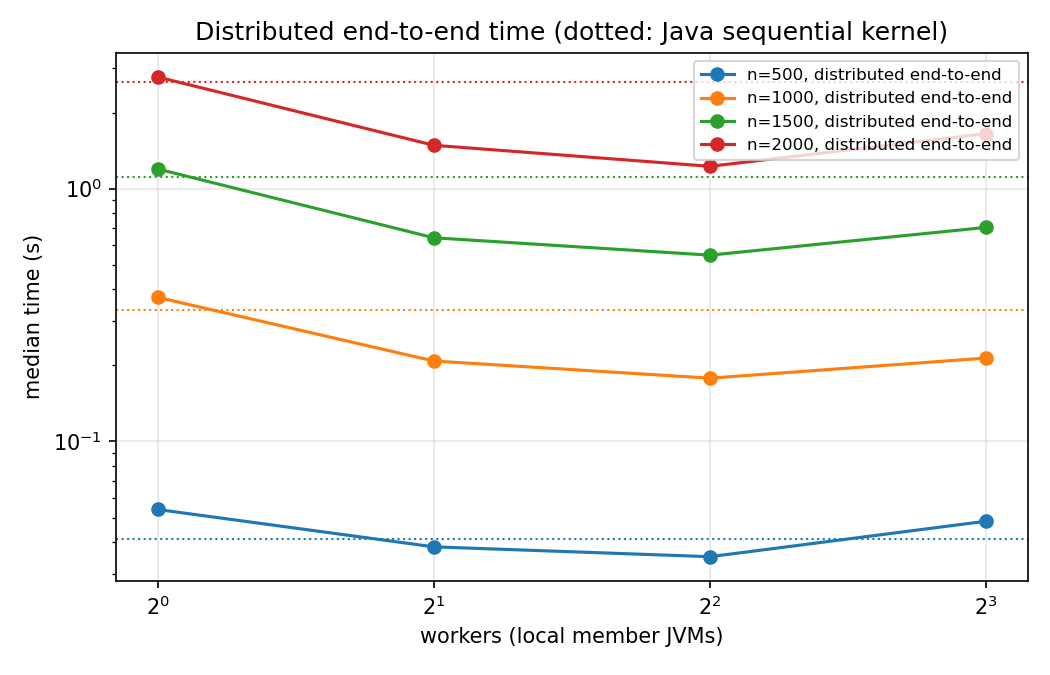
\includegraphics[width=0.82\textwidth]{figures/dist_time.png}
\caption{Median distributed end-to-end time against the number of workers (logarithmic axes); dotted lines show the Java sequential kernel time of each size.}
\end{figure}

\begin{figure}[H]
\centering
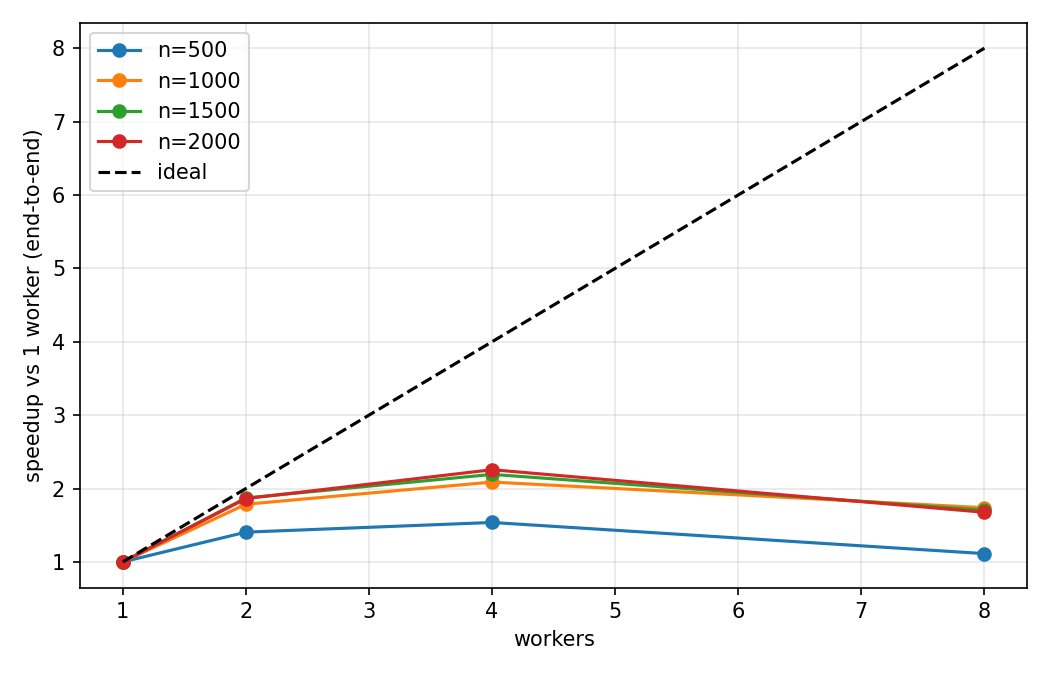
\includegraphics[width=0.82\textwidth]{figures/dist_speedup.png}
\caption{Speedup over one distributed worker (end-to-end); the dashed line is ideal speedup.}
\end{figure}

For every size, the best time is obtained with four workers and the time with eight workers is
worse than with four (by 38\% at $n=500$ and by 35\% at $n=2000$). Variability is largest with
more workers: the relative IQR is 61\% at $n=500$, $W=8$, 10.6\% at $n=1000$, $W=8$, and
5.9\% at $n=1500$, $W=4$, against at most 2.0\% for $W=1$ and $W=2$. The $n=500$, $W=8$ result should be
considered unreliable.

\subsection{Comparison with the baselines}
\begin{table}[H]
\centering
\caption{Speedup over the sequential Java kernel: distributed end-to-end time / Java threads, with the same number of workers or threads.}
\small
\begin{tabular}{@{}rrrrr@{}}
\toprule
$n$ & 1 & 2 & 4 & 8 \\
\midrule
500  & 0.77 / 1.00 & 1.08 / 1.86 & 1.18 / 3.68 & 0.85 / 4.35 \\
1000 & 0.89 / 0.99 & 1.59 / 1.76 & 1.86 / 3.36 & 1.55 / 4.97 \\
1500 & 0.93 / 0.99 & 1.75 / 1.83 & 2.04 / 3.24 & 1.59 / 4.44 \\
2000 & 0.96 / 1.00 & 1.79 / 1.79 & 2.16 / 3.06 & 1.61 / 3.88 \\
\bottomrule
\end{tabular}
\end{table}
With one worker the distributed run takes 30.3\%, 12.3\%, 7.2\% and 4.3\% more time than the
sequential kernel for $n=500,1000,1500,2000$. The kernel time measured inside the task with
one worker is within 2.6\% of the sequential kernel time for all sizes. The distributed
version is never faster than Java threads with the same count: for $n=2000$, the ratio of
distributed time to threaded time is $1.04, 1.00, 1.41, 2.42$ for $1, 2, 4, 8$, and at
$n=500$ it is $1.31, 1.72, 3.12, 5.09$.

\subsection{Where the time goes}
\begin{table}[H]
\centering
\caption{Distributed phases for $n=2000$ (median seconds). Upload, compute and assemble are consecutive; the in-task times overlap the compute phase.}
\small
\begin{tabular}{@{}rrrrrrr@{}}
\toprule
$W$ & upload $B$ & compute phase & assemble $C$ & slowest $B$ read & slowest kernel & compute $-$ slowest kernel \\
\midrule
1 & 0.030 & 2.731 & 0.0019 & 0.0095 & 2.655 & 0.077 \\
2 & 0.024 & 1.458 & 0.0019 & 0.0329 & 1.374 & 0.083 \\
4 & 0.026 & 1.198 & 0.0019 & 0.0698 & 1.100 & 0.098 \\
8 & 0.093 & 1.542 & 0.0077 & 0.2868 & 1.226 & 0.316 \\
\bottomrule
\end{tabular}
\end{table}

\begin{figure}[H]
\centering
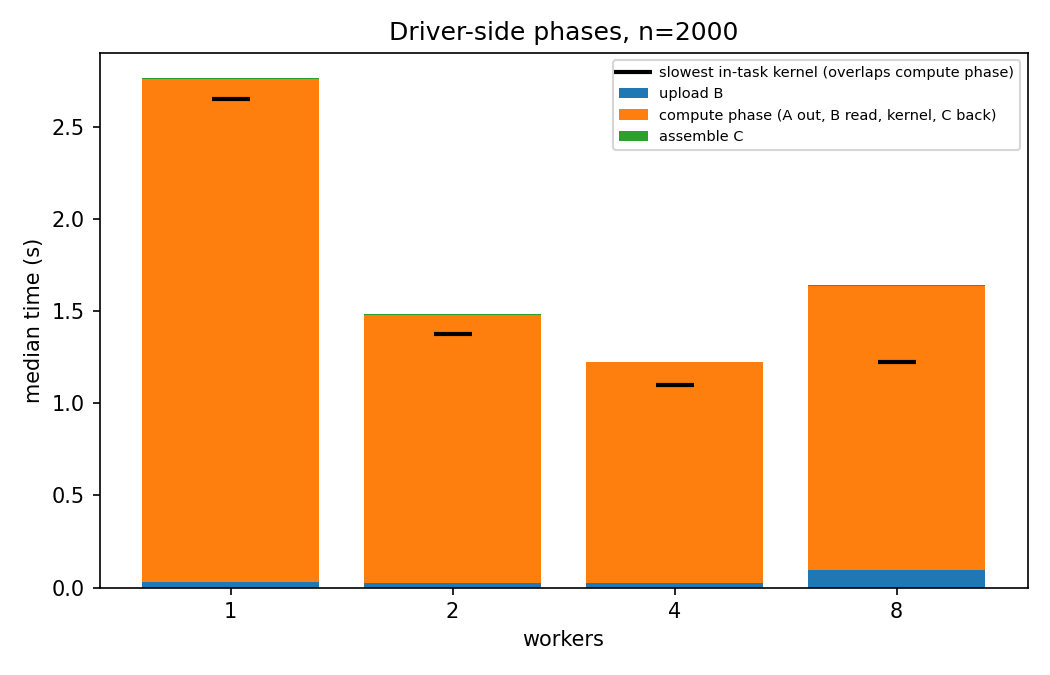
\includegraphics[width=0.82\textwidth]{figures/dist_phases.png}
\caption{Driver-side phases for the largest size ($n=2000$); the marker shows the slowest in-task kernel, which overlaps the compute phase.}
\end{figure}

The compute phase accounts for about 99\% to 98\% of the end-to-end time at $n=2000$ for
$W=1$ to $4$ and for 94\% at $W=8$; uploading $B$ and assembling $C$ are small. The
difference between the compute phase and the slowest in-task kernel (last column) is the
time that is not the slowest kernel: it includes sending the blocks of $A$, reading $B$ (up to
0.287\,s in the slowest task at $W=8$), returning $C$ and scheduling. It is not a measurement
of any single component. This difference grows with the number of workers, from 2.8\% of the
compute phase at $W=1$ to 20.5\% at $W=8$ ($n=2000$), and from 4.1\% to 24.6\% for $n=1500$.
Uploading $B$ takes 0.030\,s with one worker and 0.093\,s with eight.

The kernel itself also scales less than the number of workers. The slowest in-task kernel at
$n=2000$ is $1.93$, $2.41$ and $2.17$ times faster than with one worker for $W=2,4,8$, whereas
Java threads reach 3.06 and 3.88 times over the sequential kernel with 4 and 8 threads. At
$n=500$, where $B$ occupies 2\,MB, the slowest kernel reaches $3.66$ and $5.00$ times for
$W=4$ and $8$, while at $W=8$ the slowest task spends 0.034\,s reading $B$ against 0.0084\,s
in the kernel.

The estimated payload $(3+W)\cdot 8n^2$ bytes at $n=2000$ is 122\,MiB for $W=1$ and 336\,MiB
for $W=8$ (calculated, not measured). Loopback transfer is not representative of a network
between machines.

\subsection{Memory}
\begin{table}[H]
\centering
\caption{Sampled RSS for $n=2000$ (MiB). Total is the maximum over samples of the sum over processes; driver and member are the maxima of a single process.}
\small
\begin{tabular}{@{}lrrr@{}}
\toprule
Configuration & Total & Driver / process & Largest member \\
\midrule
seq              & 142.8 & 142.8 & -- \\
par, 1--8 threads & 142.5--144.8 & 142.5--144.8 & -- \\
dist $W=1$       & 1353.8 & 667.8 & 686.0 \\
dist $W=2$       & 2590.0 & 662.8 & 1024.2 \\
dist $W=4$       & 3048.3 & 706.9 & 762.3 \\
dist $W=8$       & 3127.2 & 510.4 & 499.2 \\
\bottomrule
\end{tabular}
\end{table}
The three matrices of $n=2000$ need $91.6$\,MiB, and the sequential and threaded runs are
close to this plus the JVM (about 143\,MiB). The distributed driver samples at 510--707\,MiB
and each member at 499--1024\,MiB, so the total across processes is 9.5 times (one worker)
to 21.9 times (eight workers) the sequential value, and 3127\,MiB at $W=8$ is about 38\% of
the 8\,GB of RAM. Member RSS does not decrease as the number of workers increases: every task
assembles its own full copy of $B$, serialization creates temporary buffers, and the JVM
keeps heap it has grown. Values near 1\,GiB (982\,MiB at $n=1500$, $W=2$, and 1024\,MiB at
$n=2000$, $W=2$) are close to the configured heap limit of 1\,GiB per member; the effect
of this on the times was not assessed. The sampled values for the threaded runs at $n=500$
with 4 and 8 threads (2.2\,MiB) are implausible for a JVM holding the matrices and are most
likely a sampling artefact of a very short run; they are not used. Full values are in
\texttt{memory.csv}.

% ------------------------------------------------------------------ 5
\section{Discussion}
\paragraph{Scaling inside the framework.} With two workers the distributed version scales
well for $n\ge1000$ (efficiency 0.89--0.94), and with four workers the speedup is 2.1--2.3
for $n\ge1000$ (efficiency 0.52--0.56). Beyond four workers the time increases. The eight
members and the driver make nine JVM processes on eight execution contexts, so $W=8$ is
oversubscribed, and four of the cores are efficiency cores; macOS offers no way to pin
processes, so placement was not controlled. These facts are consistent with the loss at
$W=8$ but were not isolated by an experiment.

\paragraph{Overhead.} With one worker the cost over the sequential kernel is mostly the
fixed cost of moving data and scheduling: 30.3\% at $n=500$, where the kernel lasts 41\,ms,
and 4.3\% at $n=2000$. The relative overhead falls as the amount of computation per byte moved
increases, which agrees with the $O(n^3)$ versus $O(n^2)$ argument of the introduction. As the
number of workers grows, the part of the compute phase that is not the slowest kernel grows
(Table~6), and each of the $W$ tasks reads the whole of $B$, so the data read by the cluster
grows in proportion to $W$.

\paragraph{Distributed against threads.} The distributed version is not faster than Java
threads for any size or any worker count. This is the expected outcome for a single machine,
since workers in separate processes pay for serialization and inter-process communication that
threads avoid, and the hypothesis in the introduction is supported by the measurements. The
gap grows with the number of workers.

\paragraph{Kernel scaling.} The kernel of separate processes scales worse than the same kernel
in threads for $n\ge1000$ (Section~\ref{sec:results}). A possible explanation is that each
member holds its own copy of $B$ while threads share one, which increases memory traffic as the
number of workers grows; at $n=500$ the matrices are small and the kernel does scale. This
hypothesis was not tested, for example by measuring memory traffic or by running the
processes with a smaller $B$. The efficiency-core and oversubscription effects mentioned above
can also contribute.

\paragraph{Whether the results would carry to a real cluster.} In a cluster of several
machines the data would travel over a network with lower bandwidth and higher latency than the
loopback interface, and each machine would have its own memory; the overhead here may therefore
under- or over-estimate the real cost. Nothing in this study measures that.

% ------------------------------------------------------------------ 6
\section{Limitations}
\begin{itemize}
  \item Local execution only: all workers share one CPU, memory and operating system, and the
        network is loopback. The study does not show inter-machine network performance or
        multi-machine memory capacity.
  \item Only strong scaling was studied. Weak scaling was not.
  \item The largest tested size was $n=2000$, which was also the largest attempted. All
        configurations finished within the 300-second budget and none failed
        (\texttt{failures.csv} contains only its header). Larger sizes were not tried; the
        sampled total of 3127\,MiB at $n=2000$, $W=8$ is about 38\% of the RAM.
  \item Five repetitions give a limited estimate of variability; with eight workers the
        IQR is large (61\% of the median at $n=500$).
  \item The runs were made on battery power; whether power management affected them was not
        recorded.
  \item Data transfer was not measured; only an analytical payload estimate is given.
  \item Memory is sampled RSS every 0.2\,s, not true peak memory, and the heap limit of
        1\,GiB per member may have influenced some member values.
  \item Process placement on performance and efficiency cores was not controlled.
  \item Only one data layout was tested (one row block of $A$ per worker, $B$ read in full by
        every task); other partitionings (for example blocking in both dimensions) or
        data-aware task placement were not tried.
  \item The Java version (25) is newer than the Hazelcast release used (5.3.8) and warnings
        were printed; the effect on performance was not evaluated.
\end{itemize}

% ------------------------------------------------------------------ 7
\section{Conclusions}
In this local experiment, the Hazelcast implementation produces correct results (identical to
the sequential kernel) and reduces the time of a fixed problem when two to four workers are
used, with a best speedup of $2.26\times$ over one worker and $2.16\times$ over the sequential
Java kernel (both at $n=2000$, $W=4$). The overhead of the framework with one worker is
between 4.3\% and 30.3\% and falls as the size increases. Eight workers on eight execution
contexts, plus the driver, give worse times than four. The distributed version never
outperformed Java threads on the same machine and used between 9.5 and 21.9 times more
sampled memory than the sequential run at $n=2000$. What remains unresolved is how much of the
loss of scaling comes from memory traffic, from the heterogeneous cores or from oversubscription,
and how these results would change on several machines connected by a real network.

% ------------------------------------------------------------------ 8
\section{Generative AI disclosure}
The tool used was Claude (Anthropic). It was used for planning the experimental design,
drafting the Java/Hazelcast code and the run and analysis scripts, helping with debugging, and
drafting and revising the English text of this report. The measurements were executed by the
student on her own computer, and the numbers in this report come from those runs. The student
is responsible for understanding the code, validating the measurements and the references, and
defending the conclusions.

% ------------------------------------------------------------------ 9
\section{References and materials}\label{sec:repro}
\begin{thebibliography}{9}
\bibitem{hz-exec} Hazelcast, ``Interface IExecutorService'' (Javadoc, version 5.5.0).
  \url{https://docs.hazelcast.org/docs/5.5.0/javadoc/com/hazelcast/core/IExecutorService.html}
\bibitem{hz-imap} Hazelcast, ``Interface IMap'' (Javadoc, version 5.4.0).
  \url{https://docs.hazelcast.org/docs/5.4.0/javadoc/com/hazelcast/map/IMap.html}
\bibitem{hz-map-guide} Hazelcast, ``Map'' (IMDG 4.0 reference manual, backup count).
  \url{https://docs.hazelcast.com/imdg/4.0/data-structures/map}
\bibitem{amdahl} G.~M. Amdahl, ``Validity of the single processor approach to achieving large
  scale computing capabilities,'' in \emph{Proc. AFIPS Spring Joint Computer Conf.}, 1967,
  pp.~483--485. doi:10.1145/1465482.1465560.
\bibitem{gustafson} J.~L. Gustafson, ``Reevaluating Amdahl's law,'' \emph{Commun. ACM},
  vol.~31, no.~5, pp.~532--533, 1988. doi:10.1145/42411.42415.
\bibitem{splitmix} S.~Vigna, ``splitmix64.c'' (public domain reference implementation).
  \url{https://prng.di.unimi.it/splitmix64.c}
\bibitem{course} Universidad de Las Palmas de Gran Canaria, \emph{Big Data -- Individual
  Assignments: Matrix Multiplication}, academic year 2026--2027 (assignment statement).
\end{thebibliography}

\paragraph{Materials.} Source code, scripts, raw data and figures are in the GitHub
repository, branch \texttt{assignment-4}, folder \texttt{part4/}:\\
\url{https://github.com/zayrapenya/matrix-multiplication/tree/assignment-4}

\begin{itemize}
  \item \texttt{src/main/java/mm/}: kernels and generator (\texttt{Kernels}), task executed
        by a member (\texttt{RowBlockTask}), driver and tests (\texttt{Dist}, \texttt{Bench}),
        member (\texttt{Member}) and Hazelcast configuration (\texttt{Common}).
  \item \texttt{pom.xml}: dependencies (Hazelcast 5.3.8) and shaded jar.
  \item \texttt{scripts/run\_distributed.sh}, \texttt{scripts/analyze\_results.py},
        \texttt{scripts/collect\_environment.sh}.
  \item \texttt{results/}: \texttt{raw\_benchmarks.csv} (180 measurements), \texttt{summary.csv},
        \texttt{scaling.csv}, \texttt{memory.csv}, \texttt{environment.txt},
        \texttt{test\_output.txt}, \texttt{failures.csv},
        \texttt{checksum\_crosscheck\_vs\_part3.csv}; \texttt{figures/}: generated plots.
\end{itemize}
From the repository root:
\begin{verbatim}
cd part4
mvn -q package
bash scripts/run_distributed.sh
python3 scripts/analyze_results.py
\end{verbatim}
The runner replaces \texttt{results/raw\_benchmarks.csv}, so existing results should be copied
before rerunning. Sizes, worker counts, repetitions, warm-ups, budget and heap sizes can be
changed with the environment variables \texttt{SIZES}, \texttt{WORKERS}, \texttt{THREADS},
\texttt{REPS}, \texttt{WARMUP}, \texttt{BUDGET\_S}, \texttt{MEMBER\_XMX} and
\texttt{DRIVER\_XMX}.

\end{document}
